\begin{figure}[t]
\centering
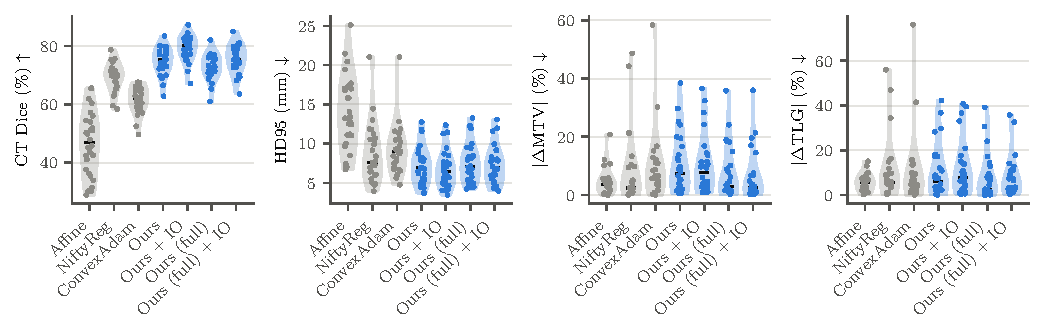
\includegraphics[width=\textwidth]{figures/baselines_distribution.pdf}
\caption{Patient-level results on the test set (28 patients; a patient's pairs are averaged). Boxes: median and interquartile range, whiskers: 1.5$\times$IQR; each dot is one patient. Initial alignment is omitted (CT Dice 9.5\,\%, HD95 44.4\,mm; MTV/TLG change 0 by construction, Table~\ref{tab:baselines}).}
\label{fig:baselines_distribution}
\end{figure}
